



\section{Results and Discussion}

%We measure the performance of proofreading quantitatively by comparing VI scores of segmentations against ground truth labelings. Lower VI scores indicate less distance to the ground truth and a better segmentation. For all experiments, we report the VI score of the initial segmentation followed by the VI score of the proofreading output.

\subsection{Classifier Comparison}

We compare the guided proofreading and focused proofreading classifiers and report precision/recall as well as f1 scores across datasets.

\paragraph{L. Cylinder.} Evaluation was performed on previously unseen sections of mouse cortex volume of Kasthuri~\etal~\cite{kasthuri2015saturated}. We generated an unbalanced dataset of 81,184 correct and 8,780 split error patches in respect to the ground truth labeling. We then ranked each patch using focused proofreading and guided proofreading and compared precision/recall (Table \ref{tab:prcyl}. Our method exhibits higher precision and recall for correct and error patches.

\begin{table}[h]
\caption{Classifier comparison on an unbalanced test set of the L. Cylinder volume.}%While the training of our classifier is more expensive, testing accuracy is superior. }

\small{
\begin{tabular}{l|c|c|c|c}

 & precision & recall & f1 score & \# \\ 
\textbf{Focused Proofreading} & ~ & ~ & ~ & ~ \\ 
correct & 0.93 & 0.31 & 0.47 & 81,184 \\ 
split error & 0.11 & 0.78 & 0.19 & 8,780 \\ 
\textbf{Guided Proofreading} & ~ & ~ & ~ & ~ \\ 
correct & 1.00 & 0.93 & 0.96 & 81,184 \\ 
split error & 0.61 & 0.96 & 0.74 & 8,780 \\ 
\end{tabular} 
}
\label{tab:prcyl}
\end{table}

\paragraph{AC4 subvolume.} We generated 3,488 correct and 332 error patches (10 merge errors, 322 split errors). Again, guided proofreading achieves better precision/recall scores (Table \ref{tab:prac4}).

\begin{table}[h]
\caption{Classifier comparison on correct and split error patches of the AC4 subvolume.}%While the training of our classifier is more expensive, testing accuracy is superior. }

\small{
\begin{tabular}{l|c|c|c|c}

 & precision & recall & f1 score & \# \\ 
\textbf{Focused Proofreading} & ~ & ~ & ~ & ~ \\ 
correct & 0.94 & 0.69 & 0.80 & 3,488 \\ 
split error & 0.14 & 0.51 & 0.21 & 332 \\ 
\textbf{Guided Proofreading} & ~ & ~ & ~ & ~ \\ 
correct & 1.00 & 0.92 & 0.96 & 3,488 \\ 
split error & 0.54 & 0.95 & 0.69 & 332 \\ 
\end{tabular} 
}
\label{tab:prac4}
\end{table}

\subsection{Forced Choice User Experiment}
We performed a user study to evaluate the forced choice error correction method among novices and experts. To perform a reasonable experiment and be comparable to Haehn's~\etal Dojo user study, participants were asked to proofread the AC4 subvolume for 30 minutes. Even with computer-aided proofreading methods, correcting the whole volume in this time frame is simply not possible. We counted 10 merge errors and 322 split errors by computing the maximum overlap of the initial segmentation and the ground truth labeling (both provided by Haehn~\etal). For evaluation, we measure the performance of proofreading quantitatively by comparing VI scores of proofread segmentations against the ground truth labelings. The median VI of the initial segmentation in respect to ground truth was 0.476 (SD=0.089). Most novices and all experts were able to improve this with focused proofreading and guided proofreading (Fig.~\ref{fig:ac4trails}).

\paragraph{Novice performance.} Participants using focused proofreading were able to reduce the median VI of the automatic segmentation to 0.469 (SD=0.87). On average, users viewed 423.4 corrections and accepted 45.8 of them with an average time of 4.9 seconds spent per correction. Participants using guided proofreading were able to reduce the median VI to 0.424 (SD=0.037). Here, users viewed 353.4 corrections on average and accepted 106.9 in 6.2 seconds. While three users of focused proofreading made the initial segmentation worse, all participants using guided proofreading were able to improve it. In comparison to the results of Haehn~\etal, focused and guided proofreading outperform interactive proofreading with Dojo. The slope of VI per correction in Fig.~\ref{fig:ac4trails} shows that guided proofreading enables VI changes with fewer corrections. Interestingly, the performance decreases after approximately 300 corrections. There are two explanations for this: user fatigue and increasing uncertainty during error suggestion from the classifier. Regarding fatigue, we suggest for future experiments to add short breaks after every ten minutes.

\paragraph{Expert performance.} Domain experts were able to improve the initial segmentation in all cases. With focused proofreading, the median VI of the automatic segmentation was 0.439 (SD=0.084). With guided proofreading, the median VI was 0.396 (SD=0.032) as shown in Fig.~\ref{fig:ac4boxplot}.

\paragraph{Subjective responses.} All subjective responses were recorded using the NASA-TLX workload index. Mental, physical, and temporal demands were reported slightly higher for participants using focused proofreading. However, these differences were not statistically significant. This is not surprising since the user interface was the same for both control groups.

\subsection{Automatic Error Correction}

\paragraph{Selection Oracle.} Accepting and rejecting proofreading corrections with the selection oracle yields the best performance on all datasets. This is not surprising since all detected merge and split are corrected if the segmentation is improved. Fig.~\ref{fig:ac4trails} shows slope of VI reduction using the selection oracle on the AC4 subvolume. With focused proofreading, the selection oracle reaches a median VI of 0.353 (SD=0.037) after 1605 corrections. With guided proofreading, the oracle reaches a median VI of 0.342 (SD=0.03) after approximately 800 corrections and then stagnates until all regions are proofread. Both results are very close to the best possible median VI of 0.334 which we calculated by computing maximum overlap with the ground truth. The slope of the trails in Fig.~\ref{fig:ac4trails} shows that guided proofreading requires less corrections to reach a reasonable reduction in VI on the AC4 subvolume and Fig.~\ref{fig:ac4boxplot} shows the distribution.
The results on the L. Cylinder dataset (initial VI XX (SD=YY) are similar: Focused proofreading reduces the median VI to XX (SD=YY) after 26,170 corrections. Guided proofreading reduces the median VI to XX (SD=YY) after XX corrections.

\paragraph{Automatic Method.} 

\subsection{Merge vs. Split Error Detection}

\subsection{Limitations}

\begin{figure}[t]
\begin{center}
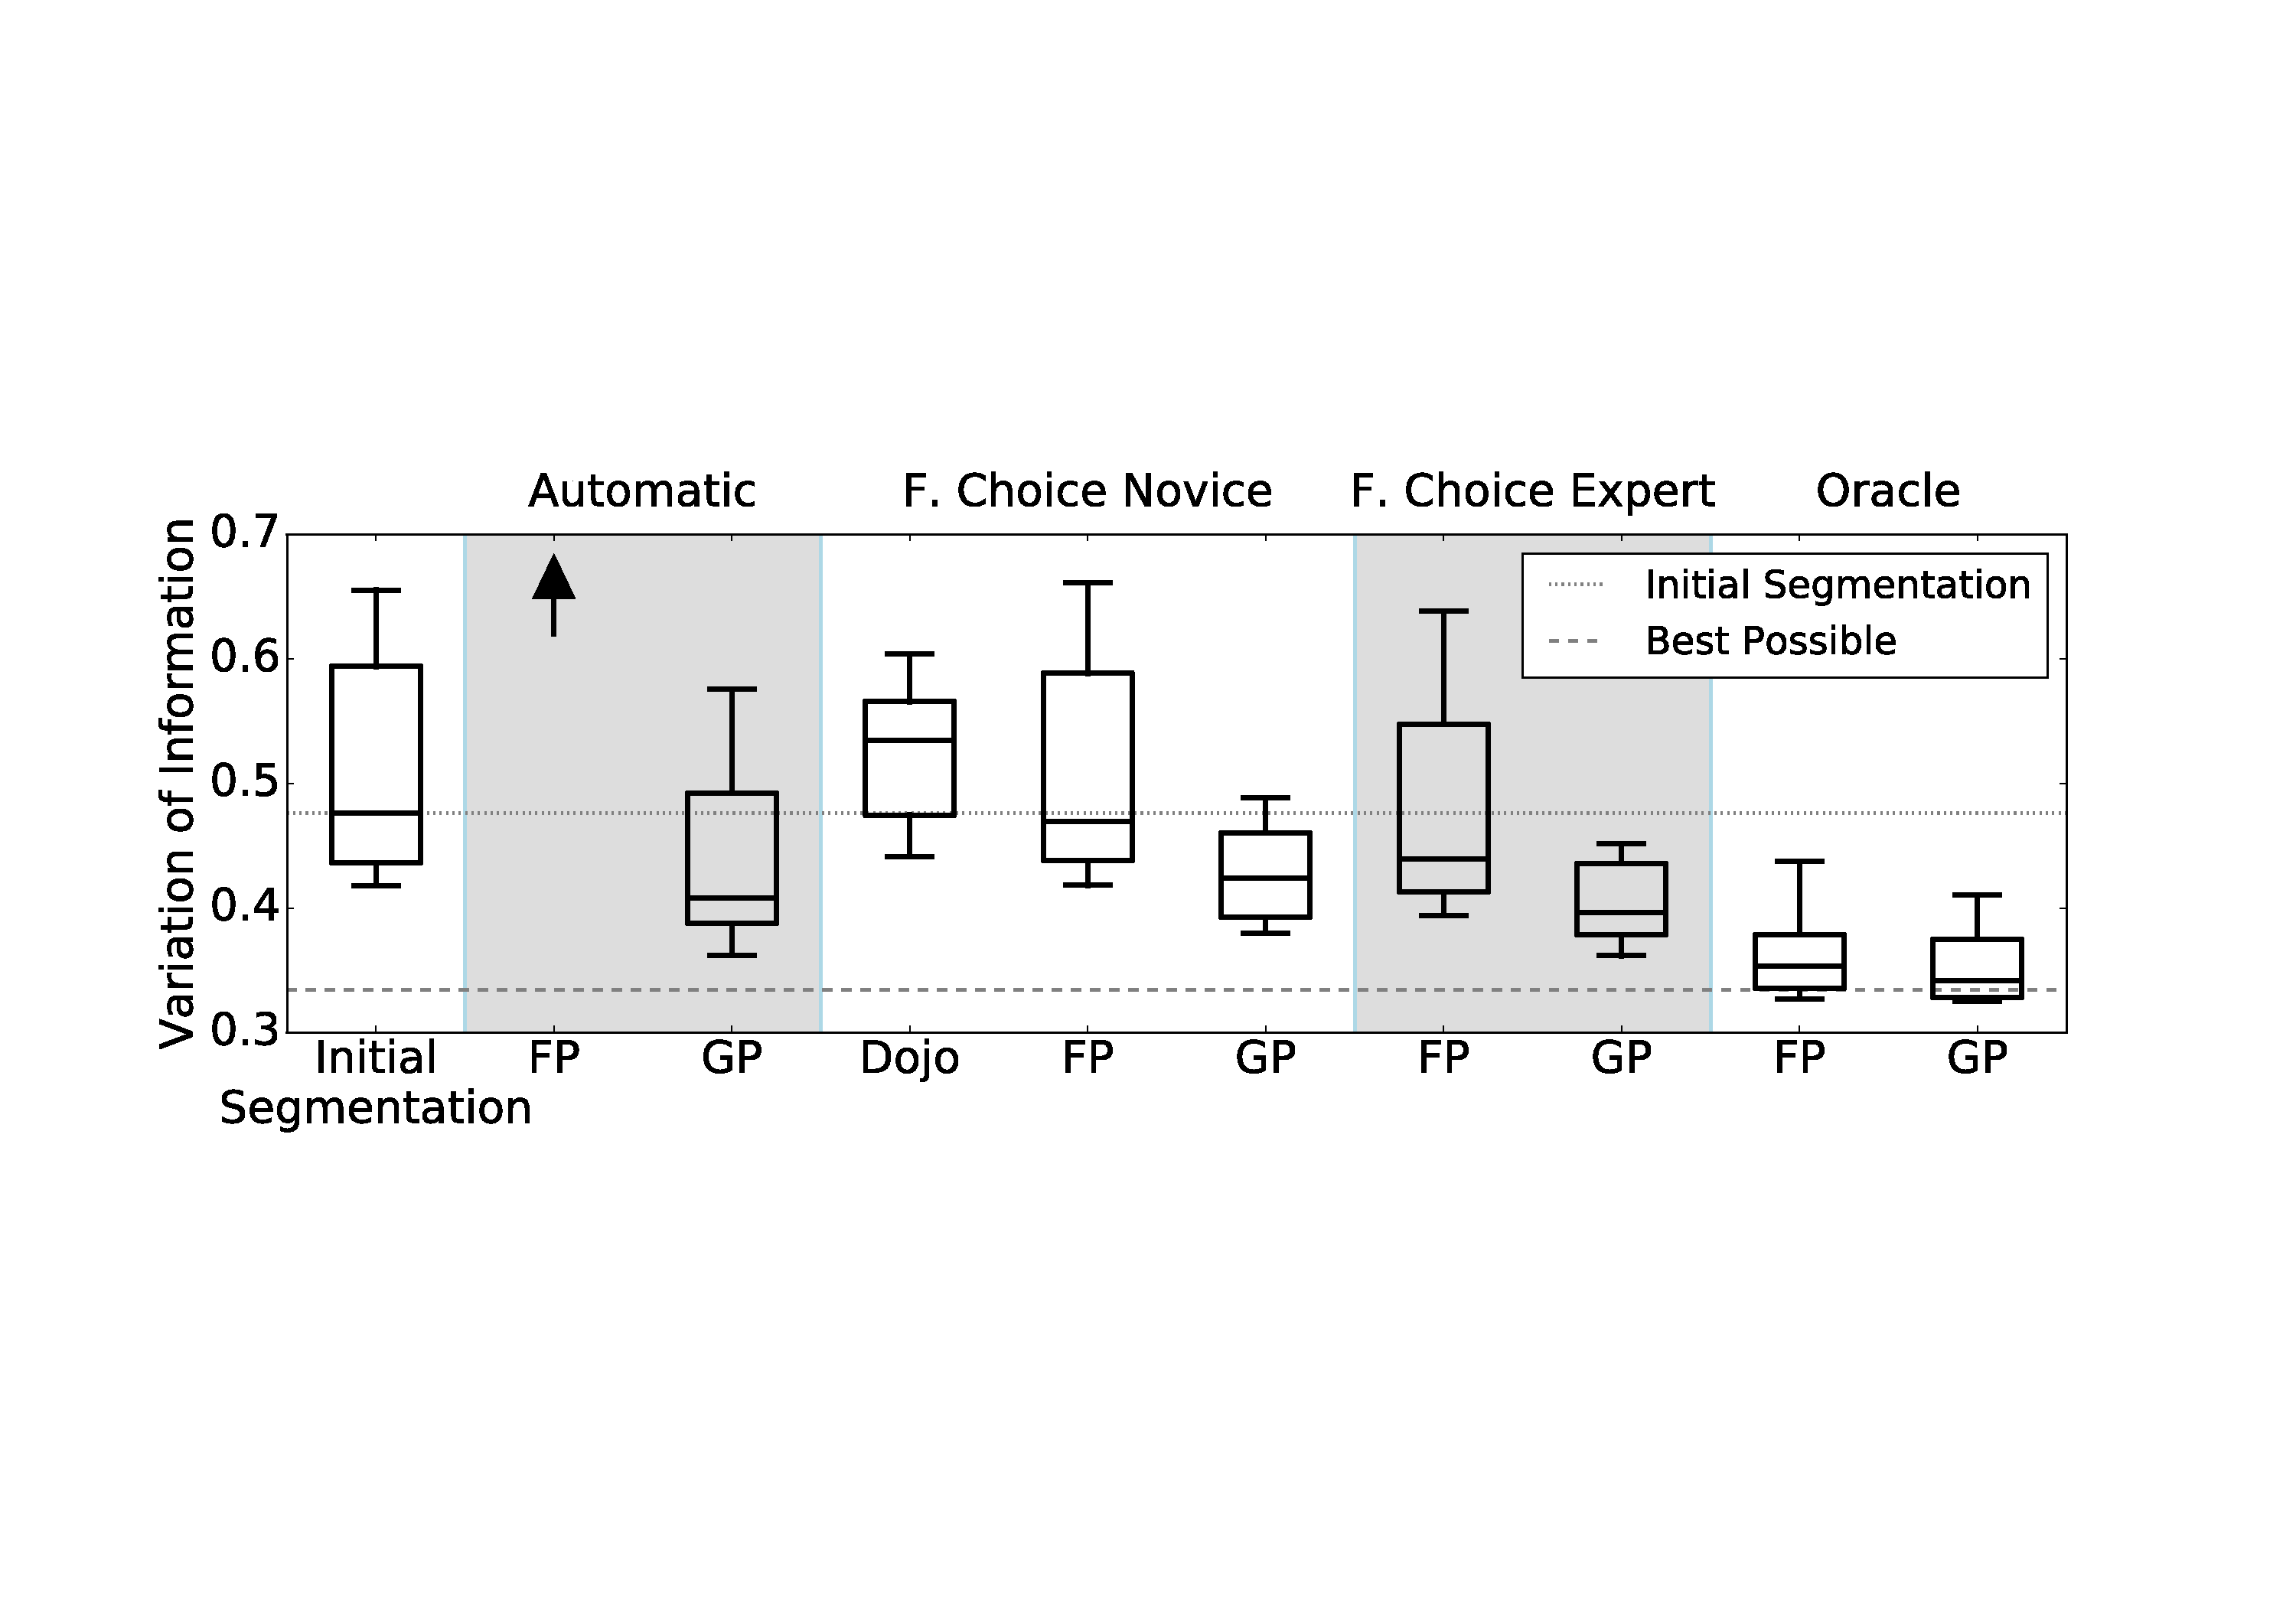
\includegraphics[width=\linewidth]{gfx/ac4boxplot.pdf}
\end{center}
  \vspace{-4mm}
   \caption{VI distributions of proofreading output across ten slices of the AC4 subvolume. The different decision approaches yield different proofreading performances.}
\label{fig:ac4boxplot}
\end{figure}